% chap5.tex

\newcommand{\BibTeX}{Bib\TeX}

\chapter{Implementation}\label{chap:refs}

\section{Introduction}

\subsection{The Graphics Pipeline}

\begin{figure}[!h]
\centering
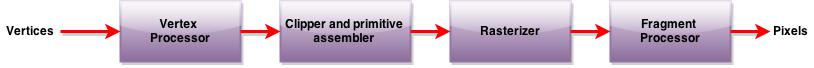
\includegraphics[width=450pt]{Images/graphics_pipeline.jpg}
\caption{\label{fig:ray_cast1.jpg} Graphics rendering pipeline overview.}
\end{figure}

In 3D computer graphics, the graphics pipeline or rendering pipeline refers to the sequence of steps used to create a 2D raster representation of a 3D scene. The figure 5.1, shows four major steps in the imaging process.

\begin{itemize}
\item \textbf{Vertex Processing:} In the first block of our pipeline, each vertex is processed independently. Here, a vertex is a set of attributes such as its location in space, as well as its color, normal, texture coordinates, amongst others. The inputs for this stage are the individual vertices attributes. The two major functions of this stage are to carry out coordinate transformations and to compute a color for each vertex. Many of the steps in the imaging process are transformations between representations of objects in different coordinate systems.

\item \textbf{Clipping and primitive assembly:} The inputs for this stage are the transformed vertices, as well as connectivity information. The connectivity information tells the pipeline how the vertices connect to form a primitive. It is in here that primitives are assembled. This stage is also responsible for clipping operations against the view frustum, and back face culling. We perform clipping because of the limitation of the viewing window size.

\item \textbf{Rasterization:} The primitives that emerge from the clipper are still represented in terms of their vertices and must be converted to pixels in the frame buffer. For example, if three vertices specify a triangle with a solid color, the rasterizer must determine which
pixels in the frame buffer are inside the polygon.

\item \textbf{Fragment processing:} The final stage in our pipeline takes in the fragments generated by the rasterizer and updates the pixels in the frame buffer. If the application generated three-dimensional data, some fragments may not be visible because the surfaces that they define are
behind other surfaces.

\end{itemize} 

Advancements in graphics cards have given programmers the ability to define the functionality of two of the above described stages: Vertex shaders for the Vertex processing stage, and fragment shaders to replace the fragment processing stage of fixed functionality.

These shaders are discussed in the next sub-sections. 


\subsection{Vertex Shader}
The Vertex Shader is the programmable Shader stage in the rendering pipeline that handles the processing of individual vertices. The vertex shader usually performs traditional graphics operations, such as, Vertex transformation, Normal transformation and normalization, Texture coordinate generation, Texture coordinate transformation, and Lighting.

The vertex shader replaces the full functionality of the vertex processor. A vertex shader is responsible for replacing all the required functionality of this stage of the pipeline, which otherwise was taken care by fixed pipeline vertex transformation stage.

\subsection{Fragment Shader}
The Fragment shader is a programmable unit that operates on fragment values and their associated data. The fragment processor usually performs traditional graphics operations, such as, operations on interpolated values, Texture access, Texture application, and fog.

Fragments are per-pixel data structures that are created by the rasterization of graphics primitives. A fragment contains all the data necessary to update a single location in the frame buffer. Fragment processing consists of the operations that occur on a per-fragment basis, most notably reading from texture memory and applying the texture value at each fragment.

The inputs for this unit are the interpolated values computed in the previous stage of the pipeline such as vertex positions, colors, normals, etc. The fragment processor operates on single fragments, i.e. it has no clue about the neighboring fragments. One important point is that a fragment shader can not change the pixel coordinate, as computed previously in the pipeline. Vertex processor (using modelview and projection matrices) can be used to transform the vertex. The fragment shader has access to the pixels location on screen but it can not change it.

\subsection{OpenGL Shading Language}

GLSL is a high-level graphics programming language formally called the openGL shading langugage. With the OpenGL Shading Language, the fixed functionality stages for vertex processing and fragment processing have been augmented with programmable stages that can do everything the fixed functionality stages can do and a whole lot more. The OpenGL Shading Language allows application programmers to express the processing that occurs at those programmable points of the OpenGL pipeline.

In OpenGL Shading Language data flows from the application to the vertex processor, on to the fragment processor, and ultimately to
the frame buffer. The OpenGL Shading Language was carefully designed to allow hardware implementations to perform parallel processing of both vertices and fragments. This parallel processes run on a hardware called Graphics Programming Unit(GPU).


\subsection{GLSL Setup for Execution}

\begin{figure}
\centering
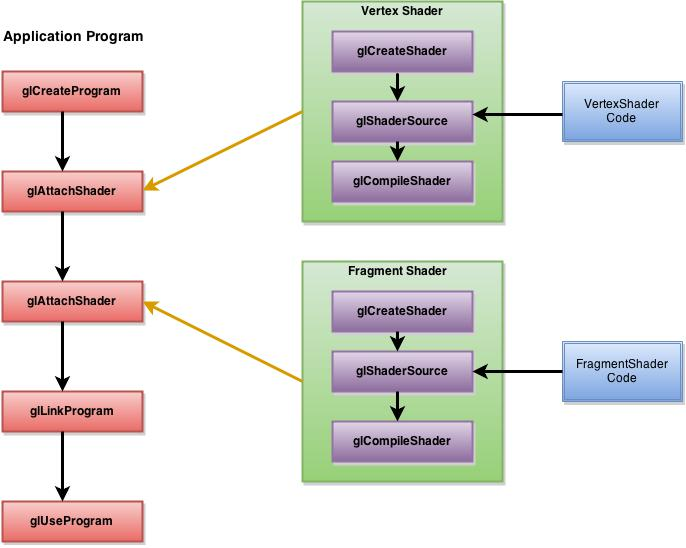
\includegraphics[width=450pt]{Images/glsl_setup.jpg}
\caption{\label{fig:ray_cast1.jpg} OpenGL GLSL program setup.}
\end{figure}
 
Every openGL Shading Language application, no matter how simple, must provide both a vertex shader and a fragment shader. Setting up the shaders requires a number of steps, including reading the shader code from files, compiling the code, and linking the shaders with the application. There is a set of openGL functions that deals with how to create vertex and shader objects, link them with an OpenGL applications, and enable the passing of variables among the OpenGL program and the shaders. As depicted by the figure 5.2, there are usually eight steps in initializing one or more shaders in the applications:

\begin{itemize}
\item Read the shader code
\item Create a program object.
\item Create shader object.
\item Attach the shader object to the program object.
\item Compiler the shaders.
\item Link everything together.
\item Select current program object.
\item Align uniform and attribute variables between the application and the shaders.
\end{itemize}

\section{Communication to GPU Shaders}

An application in OpenGL has several ways of communicating with the shaders, few are discussed below: 

\begin{itemize}
\item \textbf{Uniform Buffer Objects} are global GLSL variables declared with the "uniform" storage qualifier. Uniforms are so named because they do not change from one execution of a shader program to the next within a particular rendering call. 

\item \textbf{Buffer Textures} is a one-dimensional texture whose storage comes from a Buffer Object. They are used to allow a shader to access a large table of memory that is managed by a buffer object.

\item \textbf{Shader Storage Buffer Objects} They are a lot like uniform buffers, with their syntax almost identical to that of uniform buffer blocks. The principle difference is that you can write to them. One issue with them is that their minimum size is 16MB.


The above techiques enables flow of data from application program to GPU shaders. But the only way to obtain output from shaders to the  application program, is to render to some targets, usually the color and depth buffers. 

\end{itemize}

\section{Datasets}

Datasets used were taken from www.volvis.org, which is publicly available. All datasets used are in RAW binary format. For multimodal visualization, we have used a fabricated PET dataset.

\begin{table}
\centering
\caption{Dataset details}
\label{tab:pop}
\vspace{2mm}
\begin{tabular}{|c|c|}
\hline
Dataset & Dimension \\
\hline
Foot & 256x256x256x1 \\
\hline
Stent & 512x174x512x1 \\
\hline
head & 256x256x256x1 \\
\hline
\end{tabular}
\end{table} 


\section{Two-pass Rendering}

In the implementation of two pass rendering raycasting which is discussed in section 2.3.2, we make use of two pair of vertex and fragment shaders. In first pass, the first pair of shaders writes color location of cube with the front face culled, onto a 2D RGB texture. The location of the vertex is also its color which is assigned to the cube in the application program. In this first pass, the output of  vertex shader are the transformed and colored vertices of the cube,  assembled into primitives and fed into rasterizer, which then  interpolates the color values between the vertices. The fragments generated by rasterizer are sent to fragment shader, which in turn writes to a 2D RGB texture. This method of capturing images that would normally be drawn to the screen onto a 2D texture is called \textit{offscreen rendering}. This 2D RGB texture holds the clip-space coordinate which is the exit point of the ray originated from the camera.

In the second pass, the second shader pair are used to generate the final image which is rendered on a window. In this pass, 3D texture is used to store the volume data and it is sent across to shaders as uniform objects. We use texture samplers to retrieve the voxel data from the 3D texture.  Along with this, the 2D RGB texture which holds the bounding box exit point, is bound as uniform object and is used in the fragment shader. In this pass, the backface of the bounding box is culled. In the vertex shader, vertices are transformed and colored similar to first pass. The fragment shader receives fragments color from the rasterizer, this corresponds to the entry location of the ray on the bounding box. Now, we have both entry point and exit point which is obtained using 2D RGB texture. After computing the direction of the ray using entry and exit point, we start from the entry location and move towards exit location sampling values at uniform location defined by the stepsize. We use texture sampler to fetch data values from the 3D texture for the given location. The values received from the texture sampler is used for front-to-back compositing as discussed in the section 2.3.4.2.           

When compositing, we also compute the histogram as discussed in the section 3.4. The histogram computed for each ray is written to an offscreen buffer. At the application program, by summation of all texel values in the buffer we obtain the final histogram and it is displayed on a seperate window. 

\section{Graphics Pipeline in Hardware}

The graphics pipeline is well suited to the rendering process because it allows the GPU to function as a stream processor since all vertices and fragments can be thought of as independent. This allows all stages of the pipeline to be used simultaneously for different vertices or fragments as they work their way through the pipe. In addition to pipelining vertices and fragments, their independence allows graphics processors to use parallel processing units to process multiple vertices or fragments in a single stage of the pipeline at the same time.

In this thesis, we use ray casting to perform all the computations involved in visibility-guided volume rendering: computing visibility histograms and compositing for direct volume rendering. In both of these, the computations per ray are independent of other rays. Hence, the algorithm is intrinsically parallelizable and has been programmed on the GPU by implementing vertex and fragment shader as described in section 5.4. This resulted in performance that supports interactivity. 



